\chapter{Background}

\section{Time series}
A time series is a sequence of observations taken at regular time intervals.
These observations can be numerical values, categorical variables, or even text.
Time series data are commonly found in a wide range of fields, including finance, economics, health care, meteorology, and transportation.

\begin{figure}[H]
  \centering
  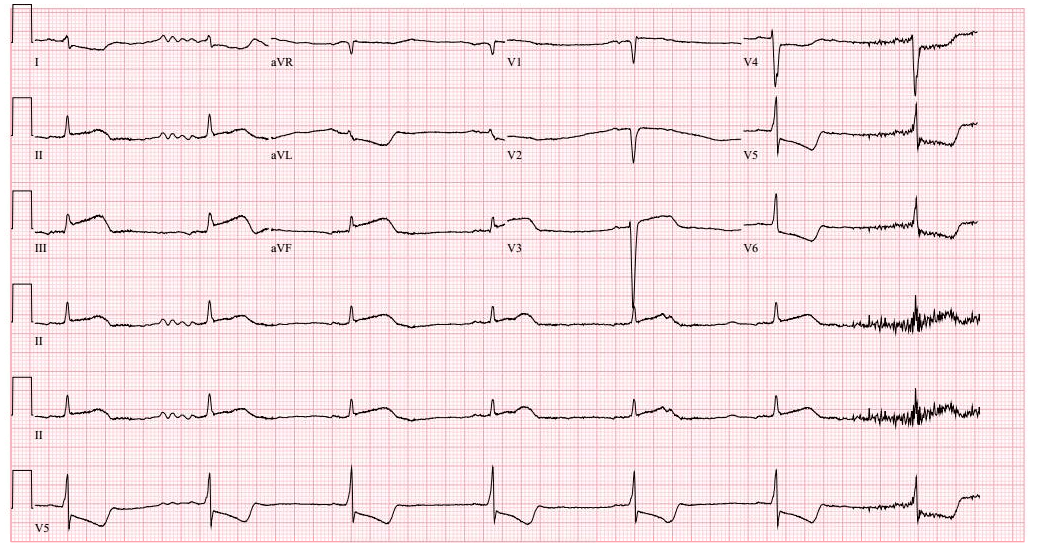
\includegraphics[width=0.45\textwidth]{hearth}
  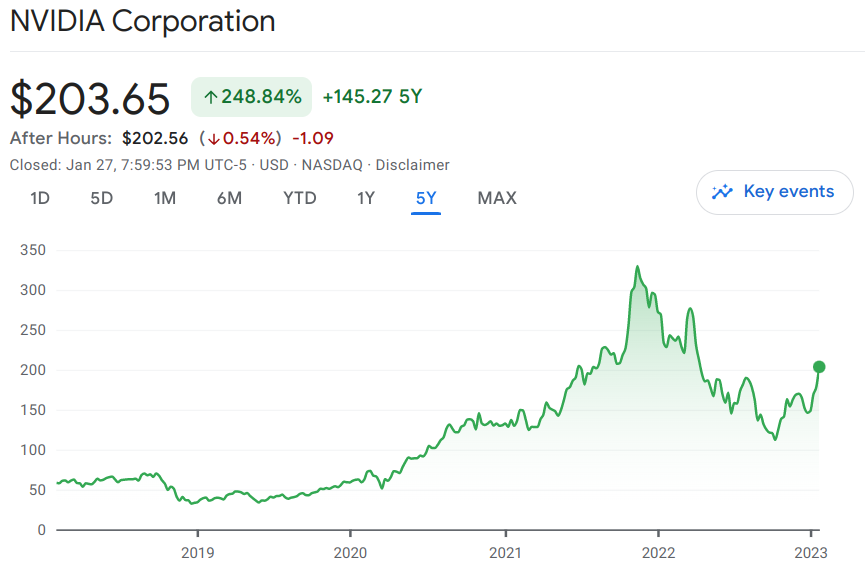
\includegraphics[width=0.45\textwidth]{nvidia}
  \caption{Example Time Series: Health Monitoring Records \cite{influxdata} and NVIDIA Stock Price \cite{finance}}
\end{figure}

In finance, for example, time series data can be used to analyze stock prices, interest rates, and currency exchange rates.
In healthcare, time series data can be used to analyze patients' vital signs, such as heart rate and blood pressure.
In transportation, time series data can be used to analyze traffic patterns and traffic flow.

\subsection{Univariate and Multivariate}

It is important to understand the difference between univariate and multivariate time series in addition to the concept of a time series.
\begin{figure}[H]
  \centering
  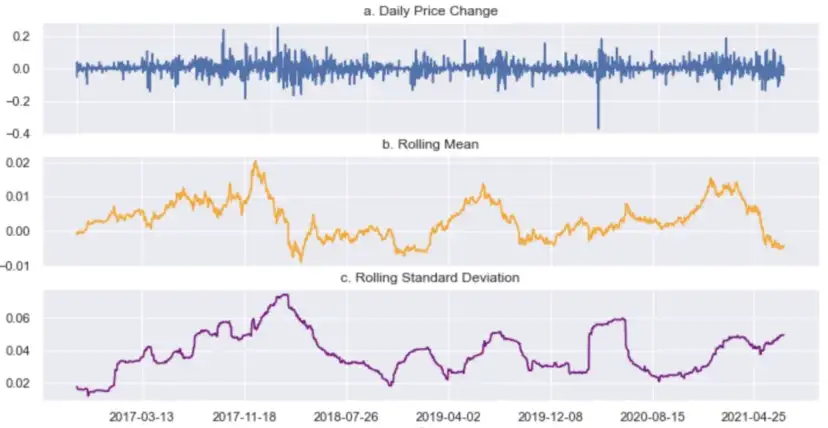
\includegraphics[width=0.6\textwidth]{multivariate}
  \caption{Multivariate Time Series Example \cite{mltech}}
\end{figure}

\paragraph{Univariate time series} This type of time series contains observations of a single variable, such as stock prices or temperature. The focus is on understanding patterns and trends in the single variable over time.
\paragraph{Multivariate time series} This type of time series includes observations of multiple variables, also known as features, over time. The main focus is on understanding the relationships and interactions between the multiple variables.

Univariate time series focus on understanding the patterns and trends of a single variable over time. This can be done by analyzing the data using techniques such as time series decomposition, trend analysis, and forecasting.
Multivariate time series, on the other hand, focus on understanding the relationships and interactions between multiple variables. 
It's important to note that the choice of model and the methods used to analyze the data depend on the type of time series data you're working with. Univariate and multivariate time series require different approaches and techniques to analyze.

\subsection{Satellite Image Time Series (SITS)}

Satellite Image Time Series (SITS) refers to a collection of satellite images taken at regular intervals over a specific area of interest. 
SITS data are obtained using remote sensing satellites that capture images of the Earth's surface at different wavelengths of the electromagnetic spectrum.

The European Union's Sentinel program is an example of a satellite mission that provides high quality SITS data with a long revisit time.
The Sentinel satellites acquire images at different spatial resolutions, ranging from 10 meters to 60 meters, depending on the mission. 
These images are acquired at different time intervals, ranging from a few days to several months, providing a time series of images for a given area.

To obtain SITS data, multiple images are taken at regular intervals over a specific area of interest. 
After the images are acquired, they go through a pre-processing step where they are aligned to a consistent coordinate system. 
This step ensures that each pixel in the time series corresponds to the same location on the Earth's surface, allowing accurate analysis and comparison of the data.

% \subsection{Spatio-temporal autocorrelation}
% Spatio-temporal autocorrelation \cite{doi:10.1080/10095020.2019.1643609} refers to the correlation between observations that are close in both space and time. 
% It is a common phenomenon in many natural and social phenomena, such as weather patterns, crime rates, and population density.

% Spatio-temporal autocorrelation can be of two types: positive and negative. 
% Positive spatio-temporal autocorrelation occurs when similar values tend to cluster together in both space and time. 
% For example, in weather patterns, regions with high temperatures tend to be near other regions with high temperatures, and this pattern tends to persist over time. 
% Negative spatio-temporal autocorrelation occurs when dissimilar values tend to cluster together in both space and time.

% Spatio-temporal autocorrelation is important to consider when analyzing spatio-temporal data, such as time series data with a spatial component.
% Ignoring spatio-temporal autocorrelation can lead to biased and unreliable results.

\section{Ensemble learning}
Ensemble learning \cite{Ho2009, Sklansky2013} is a technique in machine learning that combines multiple models to create a more powerful model.
The idea behind ensemble learning is that by combining the predictions of multiple models, the ensemble model can reduce the variance and bias of the individual models, leading to improved performance on unseen data.

There are several popular ensemble learning methods, including:

\paragraph{Bagging} This method involves training multiple models independently on different subsets of the data and then combining their predictions by majority voting or averaging.

\paragraph{Boosting} This method involves training multiple models sequentially, with each model attempting to correct the errors of the previous model. The final prediction is made by combining the predictions of all the models.

\paragraph{Random Forest} This method is a combination of bagging and decision trees. It involves training multiple decision trees independently on different subsets of the data and then combining their predictions by majority voting.

\paragraph{Stacking} This method involves training multiple models independently, and then using the predictions of those models as input features to train a meta-model.

Ensemble learning can be applied to a wide range of machine learning tasks, including classification, regression, and anomaly detection. 
It has been shown to improve performance on a wide range of datasets and is often used in practice to improve the performance of machine learning models.


\subsection{Random forests}

Random forests \cite{breiman2001random, charles2020random} are an ensemble learning method used for classification and regression tasks. 
The name ``random forest" comes from the fact that it is a collection of decision trees, where each tree is ``trained" on a random subset of the data, and the final predictions are made by combining the predictions of all the trees.

\begin{figure}[H]
  \centering
  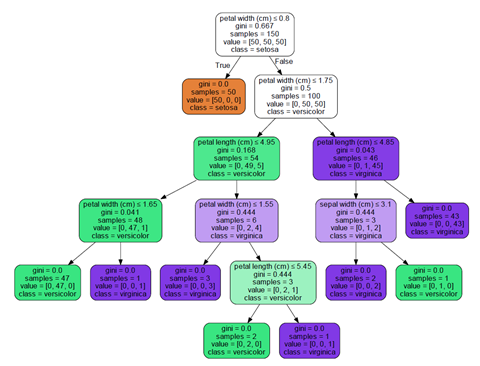
\includegraphics[width=0.8\textwidth]{decision-tree}
  \caption{Visual representation of a decision tree \cite{scikit}}
\end{figure}

A decision tree is a tree-like model that starts with a single node, called the root node, and splits the data into different subsets based on the values of the input features.
Each internal node of the tree represents a test on an input feature, and each leaf node represents a prediction.
The tree is built by recursively splitting the data until a stopping criterion is met, such as a maximum tree depth or a minimum number of samples in a leaf node.

In a random forest, multiple decision trees are trained on different subsets of the data, where the subsets are obtained by randomly sampling the data with replacement, also known as bootstrapping.
Each tree is trained on a different subset of the data, and a different subset of the input features is used at each split of the tree. 
This is known as feature bagging or random subspace method.

When making a prediction, a random forest takes the average of the predictions of all the trees for regression problems, and takes a majority vote for classification problems.
This combination of multiple decision trees reduces the variance of the individual trees and leads to improved performance on unseen data.

In summary, Random Forests are a combination of decision trees, where each tree is trained on a random subset of the data, and the final predictions are made by combining the predictions of all the trees.
This combination of multiple decision trees reduces the variance of the individual trees and leads to improved performance on unseen data.



\section{Deep learning}
Deep learning \cite{goodfellow2016deep} is a subfield of machine learning that utilizes deep neural networks, which are neural networks with multiple hidden layers, to learn from the data.
These models are capable of learning abstract features from the data and making predictions based on those features, making them particularly useful for tasks such as image and speech recognition, natural language processing, and anomaly detection.

Deep neural networks are inspired by the structure and function of the human brain, consisting of layers of interconnected nodes, also known as neurons.
The input is passed through the layers of neurons, and the output is produced at the last layer.
The layers of a neural network can be divided into three main types: the input layer, the hidden layers and the output layer.
The input layer receives the input data, and the hidden layers perform computations on the data and pass the results to the next layer. 
The output layer produces the final predictions.

Deep learning models are trained using large amounts of data and powerful computational resources, such as GPUs.
The training process involves adjusting the parameters of the model, also known as weights, to minimize the error between the predictions and the true values.
This process is known as supervised learning, where the model learns to map inputs to outputs based on labeled examples.

In recent years, deep learning has made significant advancements in various fields, including computer vision, natural language processing, and speech recognition.
The ability of deep neural networks to learn abstract features has led to significant improvements in performance on various tasks, surpassing traditional machine learning methods.

In summary, deep learning is a subfield of machine learning that utilizes deep neural networks, which are neural networks with multiple hidden layers, to model complex patterns in data.
These models are trained using large amounts of data and powerful computational resources to minimize the error between predictions and true values and have led to significant advancements in various fields.


\subsection{Perceptron}

The perceptron \cite{rosenblatt1958perceptron} is a type of artificial neural network first introduced in the 1950s by Frank Rosenblatt.
It was designed to replicate the function of a single neuron in the brain, with the ability to learn from data and make decisions based on that learning.

\begin{figure}[H]
  \centering
  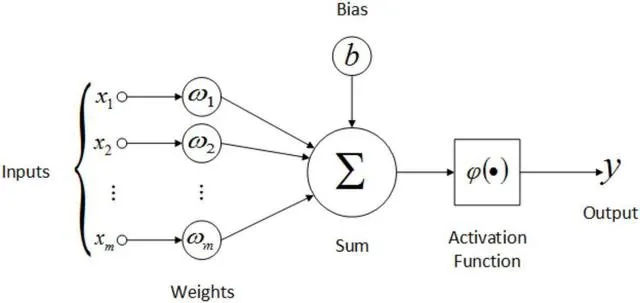
\includegraphics[width=0.6\textwidth]{perceptron}
  \caption{Perceptron Diagram \cite{Bhattacharyya}}
\end{figure}

The perceptron consists of one or more input nodes, a single output node, a bias value, and a set of weights that determine the strength of the connections between the input nodes and the output node.
The input nodes receive the input data and the weights are adjusted during training in order to make the output node produce the desired output for a given input.

The perceptron uses an activation function to determine the output of the output node. 
The activation function can be any function that maps the input to an output, but some of the most commonly used activation functions include the step function, ReLU, sigmoid, and tanh.

The perceptron can be used for binary classification problems, where the output node produces a 0 or 1 depending on the input.
It can also be used for regression problems, where the output node produces a continuous value. 
While the perceptron is a relatively simple neural network architecture, it has played an important role in the development of more complex neural networks and deep learning models.

\subsection{Activation functions}

The ReLU (Rectified Linear Unit) function, denoted as $\text{ReLU}(x)$, is defined as:

\begin{equation}
  \text{ReLU}(x) = \begin{cases}
    0 & \text{if } x < 0 \\
    x & \text{if } x \geq 0
  \end{cases}
\end{equation}

It allows for efficient computation and solves the vanishing gradient problem. 
ReLU is often used in image classification tasks.

The tanh (hyperbolic tangent) function, denoted as $\tanh(x)$, is defined as:
\begin{equation}
  \tanh(x) = \frac{\exp(x) - \exp(-x)}{\exp(x) + \exp(-x)}
\end{equation}

It is nonlinear and produces a smooth gradient, which can improve training performance. 
tanh is commonly used in recurrent neural networks for natural language processing tasks.

The sigmoid function, denoted as $\sigma(x)$, is defined as:

\begin{equation}
  \sigma(x) = \frac{1}{1 + \exp(-x)}
\end{equation}

It is a commonly used activation function in binary classification tasks because it produces a probability-like output.
Sigmoid functions can also be used in deep learning models for tasks such as object detection and speech recognition.

\subsection{Multilayer perceptrons}

Multi-layer perceptrons (MLPs) \cite{aggarwal2018neural, goodfellow2016deep} are neural networks that consist of one or more layers of perceptrons. 
These networks are also known as fully connected networks because each neuron in a layer is connected to all neurons in the next layer.

\begin{figure}[H]
  \centering
  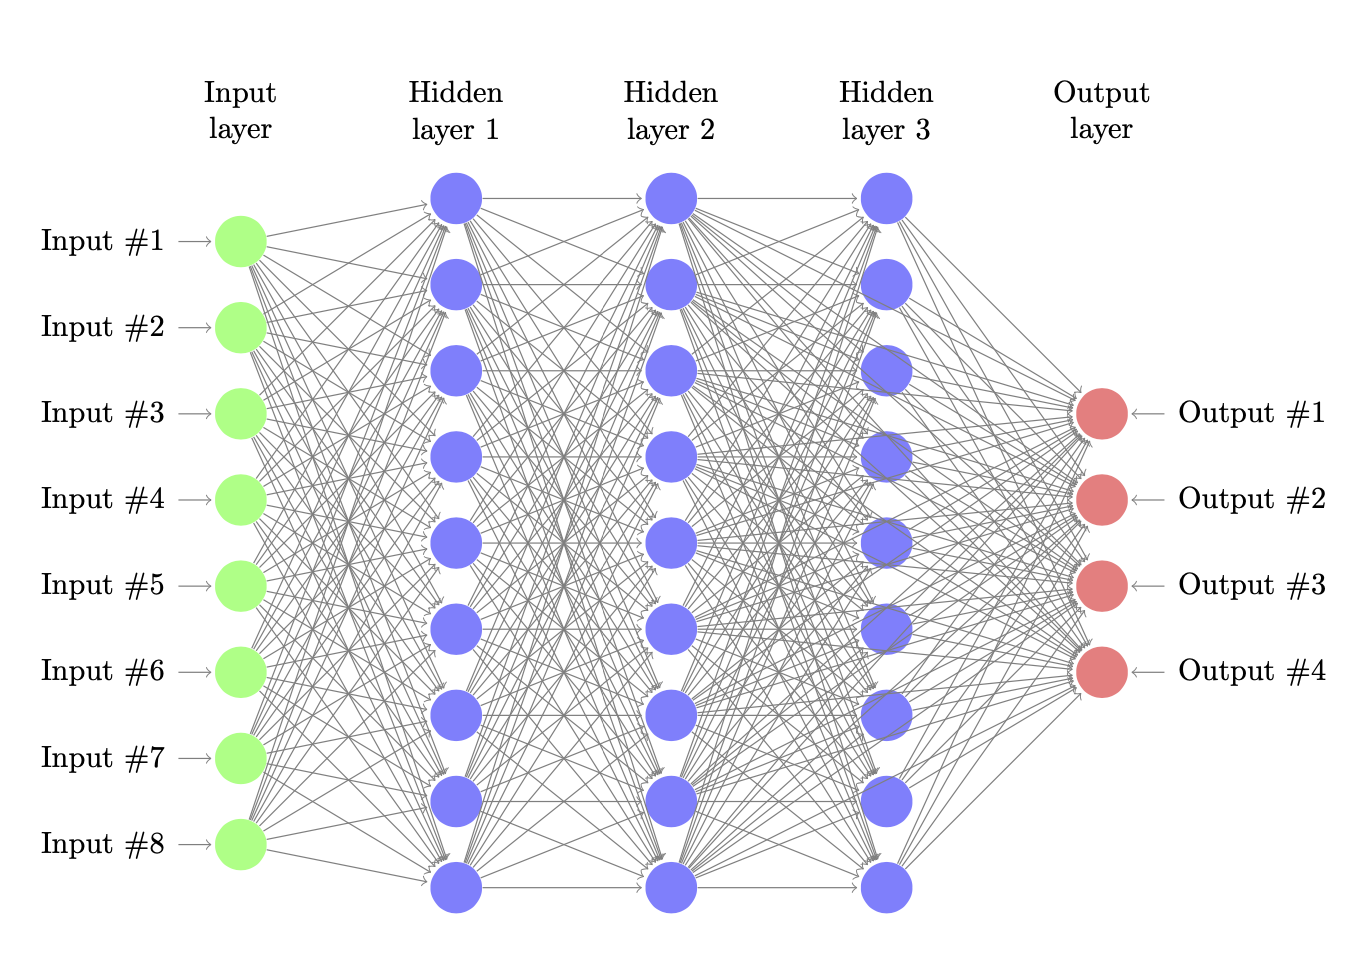
\includegraphics[width=0.8\textwidth]{mlp}
  \caption{Multilayer Perceptron (MLP) Diagram \cite{uc}}
\end{figure}

The hidden layers in an MLP allow for non-linear transformations of the input data, which can help capture complex patterns in the data that would be difficult to capture with a single perceptron. 
Each hidden layer applies a linear transformation to the inputs, followed by a nonlinear activation function, before passing the output to the next layer.

MLPs can be used for a variety of tasks, including classification, regression, and sequence prediction. 
They have been successfully applied in areas such as image recognition, natural language processing, and speech recognition. MLPs can also be used as building blocks for more complex neural networks, such as convolutional neural networks (CNNs) and recurrent neural networks (RNNs).

MLPs are trained using a process called backpropagation, which involves computing the gradient of the loss function with respect to the weights of the network, and using this gradient to update the weights through an optimization algorithm, such as stochastic gradient descent (SGD). 
The training process involves iterating over the training data multiple times, adjusting the weights of the network after each iteration, until the performance of the network on a validation set stops improving or a maximum number of epochs is reached.


\subsection{Backpropagation}

Backpropagation is a popular method for training neural networks.
It is a supervised learning algorithm that uses a form of gradient descent optimization to minimize the error between the predicted output and the actual output.
The backpropagation algorithm begins with a forward pass through the network, computing the output of each neuron layer by layer until the final output is produced.

It then calculates the error between the predicted output and the true output using a loss function.
This error is then propagated back through the network, starting from the output layer and moving backwards.
The weights of each neuron in the network are updated in the direction that reduces the error the most. 
This process is repeated until the error is minimized or a predefined stopping criterion is met.

The backpropagation algorithm requires the use of a differentiable activation function because the error must be propagated through the network to update the weights.
The choice of activation function can have a significant impact on the performance of the network, and is often the subject of experimentation and tuning.

\subsection{Loss functions}

Loss functions are used in machine learning to measure the difference between predicted output and actual output. 
The objective of a machine learning algorithm is to minimize the loss function in order to improve the performance of the model.

There are several types of loss functions, each suitable for different types of problems. For example, mean squared error (MSE) is often used in regression problems where the goal is to predict a continuous output variable.

\begin{equation}
  \text{MSE} = \frac{1}{n} \sum_{i=1}^{n} (y_i - \hat{y}_i)^2
\end{equation}

Cross-entropy loss is used in classification problems, where the output variable is discrete.

\begin{equation}
  \text{Cross-entropy loss} = - \frac{1}{n} \sum_{i=1}^{n} y_i \log(\hat{y}_i)
\end{equation}

The choice of loss function is critical in the training process of a neural network, as it can affect the performance of the model. 
It is important to choose a loss function that is appropriate for the problem at hand and that allows the model to effectively optimize its parameters.

\subsection{Batch training}
Batch training is a technique used to train neural networks using batches of samples, rather than processing the entire data set at once. 
During training, the data is divided into small batches and the model is updated after each batch is processed. 
This process helps prevent overfitting and allows for more efficient use of computational resources.

In batch training, the number of iterations over the entire dataset is typically referred to as an epoch. 
A single epoch consists of processing each batch in the training dataset once. 
After one epoch, the model has seen each training sample once and has updated weights based on the average loss across all batches in that epoch.
Multiple epochs are often used to further refine the weights and biases of the model.

The number of epochs used during training can affect model performance
Training on too few epochs can lead to underfitting, where the model has not learned enough from the data. 
On the other hand, training on too many epochs can lead to overfitting, where the model has learned too much from the training data and is unable to generalize to new data. 
Choosing the optimal number of epochs is typically done by trial and error or using early stopping techniques.

\subsection{Learning rate}
The learning rate is a hyperparameter that controls the step size of the gradient descent optimization algorithm.
It determines how much the weights of the network should be adjusted in response to error.
A high learning rate results in larger weight adjustments, while a low learning rate results in smaller weight adjustments.

\subsection{Overfitting}
Overfitting is a common problem in machine learning, where a model is trained to fit the training data too well, resulting in poor performance on new, unseen data.

Regularization is a technique used to prevent overfitting by adding a penalty term to the loss function.
This penalty term discourages the model from assigning too much importance to any one feature, and instead encourages it to find simpler, more generalizable solutions.
There are several types of regularization techniques, including L1 and L2 regularization, which add the absolute values and squared values of the weights, respectively, to the penalty term.

Dropout is another regularization technique that randomly drops a certain percentage of the neurons in a layer during training. 
This forces the remaining neurons to learn more robust features and prevents over-reliance on any one neuron. 
Dropout has proven to be an effective technique for reducing overfitting in deep neural networks.



\subsection{Convolutional neural networks}
Convolutional Neural Networks (CNNs) \cite{goodfellow2016deep} are a class of deep neural networks specifically designed to process data with a grid-like structure, such as images.
CNNs are composed of multiple layers, including convolutional layers, pooling layers, and fully connected layers.


\begin{figure}[H]
  \centering
  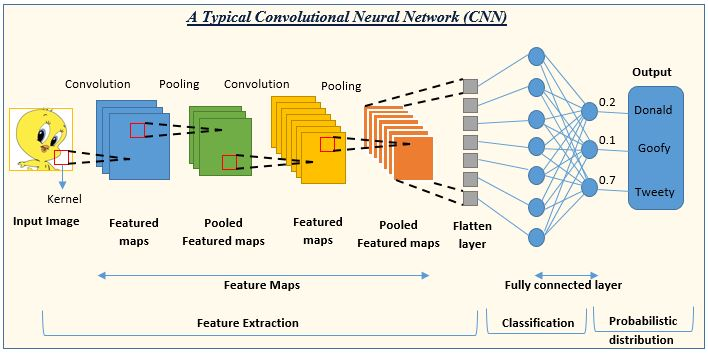
\includegraphics[width=0.8\textwidth]{cnn}
  \caption{Convolutional Neural Network (CNN) Diagram: A visual representation of a deep learning architecture consisting of layers of convolutional, pooling and fully connected layers. \cite{shah}}
\end{figure}

The convolutional layer is the core component of a CNN.
It applies a set of learnable filters to the input data, which are used to extract features from the data.
These filters are convolved with the input data, resulting in a set of feature maps.
These feature maps are then passed on to the next layer for further processing.

\begin{figure}[H]
  \centering
  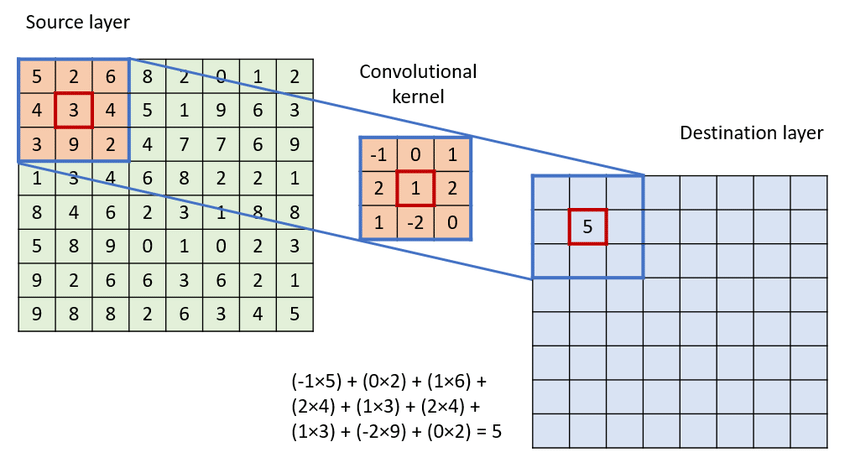
\includegraphics[width=0.8\textwidth]{conv1}
  \caption{Schematic illustration of a convolutional operation. The convolutional kernel shifts over the source layer, filling the pixels in the destination layer. \cite{convolutional:operation}}
\end{figure}

\begin{figure}[H]
  \centering
  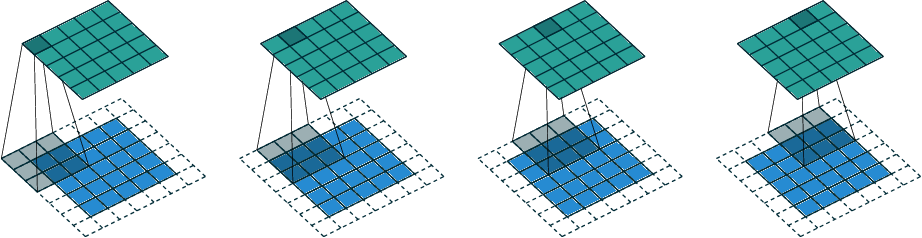
\includegraphics[width=0.8\textwidth]{conv2}
  \caption{Convolving a 3×3 kernel over a 5×5 input using half padding
  and unit strides (i.e., i=5, k=3, s=1 and p=1) \cite{arxiv.1603.07285}}
\end{figure}

Pooling layers are used to reduce the dimensionality of the feature maps and extract the most important features to increase the robustness of the network.
Max pooling and average pooling are two types of pooling layers that are commonly used. 

\begin{figure}[H]
  \centering
  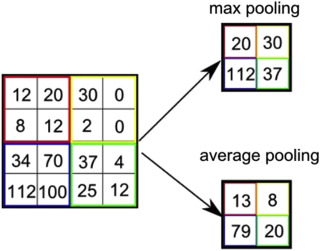
\includegraphics[width=0.4\textwidth]{pooling}
  \caption{Visualization of max and average pooling layers \cite{boehmke}}
\end{figure}

Max Pooling selects the maximum value from a small region of the input data.
This operation is used to capture the most important feature in the region, such as the strongest edge or the highest intensity value.
Max-pooling is often used in image recognition tasks because it is able to extract the most salient features from the input image, such as edges and textures.

Average pooling, on the other hand, takes the average value from a small region of the input data. 
This operation is used to reduce noise and smooth out small variations in the input data. 
Average pooling is often used in tasks such as image segmentation because it is able to extract more subtle features from the input image, such as shapes and textures.

Both have different advantages and are used in different tasks.
Many CNNs use both maximum and average pooling in different layers.


Fully connected layers are used to classify the features extracted by the convolutional layers.
They take the output of the pooling layers and use it as input to a traditional feedforward neural network, which makes the final prediction.

CNNs have been successful in a wide range of image classification tasks and have been used to achieve state-of-the-art performance on benchmarks such as the ImageNet dataset.
They have also been applied to other domains, such as video analysis and natural language processing.

One of the key advantages of CNNs is their ability to learn spatially hierarchical representations of the data.
By using convolutional layers, CNNs can learn local patterns of the data and then compose these local patterns to form more complex patterns.
This is in contrast to traditional feedforward neural networks, which use fully connected layers and are not able to take advantage of the spatial structure of the data.

Another advantage of CNNs is their ability to learn translation-invariant representations of the data.
By using pooling layers, CNNs can learn representations that are robust to small translations of the input data.
This is important for tasks such as image classification, where the object of interest may be in different locations within the image.

In summary, convolutional neural networks (CNNs) are a class of deep neural networks specifically designed to process data with a grid-like structure, such as images.
CNNs are composed of multiple layers, including convolutional layers, pooling layers, and fully connected layers.
CNNs have been successful in a variety of image classification tasks and have been used to achieve state-of-the-art performance on benchmarks such as the ImageNet dataset.
They have also been applied to other domains such as video analysis and natural language processing.
CNNs are capable of learning spatially hierarchical representations of the data and translation-invariant representations of the data.

\subsection{Temporal convolutional neural networks}

Temporal Convolutional Networks (TCNs) are a variation of CNNs that are designed to process sequential data, such as time series or videos.
They are similar to traditional CNNs in that they use convolutional layers to extract features from the input data, but they also incorporate temporal information by using dilated convolutions.

Dilated convolutions are similar to standard convolutions, but they have a dilation factor that controls the spacing between the elements of the convolutional kernel.
This allows TCNs to increase the receptive field of the network without increasing the number of parameters.
As a result, TCNs can capture long-term dependencies in the input data.

\begin{figure}[H]
  \centering
  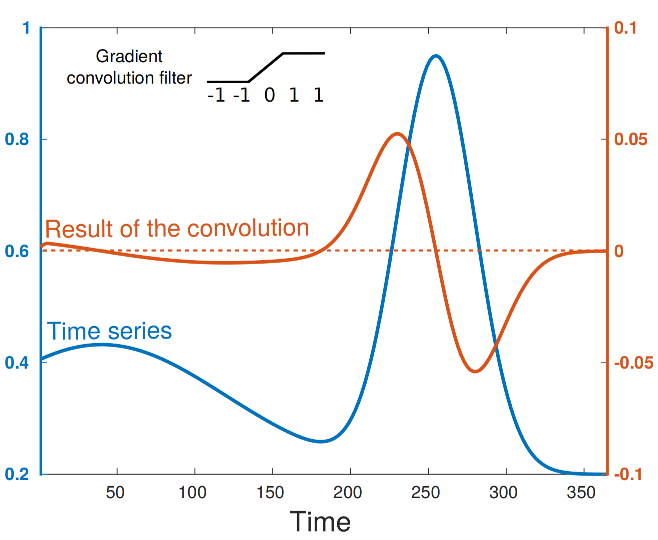
\includegraphics[width=0.7\textwidth]{temporalConvolution}
  \caption{Convolution of a time series (blue) with the positive gradient filter [-1 -1 0 1 1] (black).The result (red) takes high positive values when the signal sharply increases, and conversely\cite{tempCNN}}
\end{figure}

TCNs also use causal convolution, which means that the network's output depends only on past inputs.
This is important in tasks such as prediction, where the future cannot be influenced by the current output.

TCNs have been used in a variety of tasks, including speech recognition, natural language processing, and time series forecasting.
They have been shown to be effective in capturing temporal dependencies and have achieved state-of-the-art performance on benchmarks such as the Wall Street Journal corpus for speech recognition.

In summary, Temporal Convolutional Networks (TCNs) are a variant of CNNs designed to process sequential data, such as time series or video.
They incorporate temporal information by using dilated convolutions and causal convolution, which allows TCNs to increase the receptive field of the network without increasing the number of parameters and to capture long-term dependencies in the input data.
TCNs have been used in a variety of tasks and have been shown to be effective at capturing temporal dependencies, achieving state-of-the-art performance on benchmarks.

\subsection{Recurrent neural networks}

Recurrent Neural Networks (RNNs) \cite{graves2013generating, goodfellow2016deep} are a type of neural network designed to process sequential data, such as time series or natural language.
They are called "recurrent" because they have a feedback loop that allows information to flow from one step of the sequence to the next.

RNNs have a hidden state, which is a vector containing information about past inputs.
At each time step, the input is combined with the hidden state to produce a new hidden state and an output.
The hidden state is then used as the input for the next time step.

\begin{figure}[H]
  \centering
  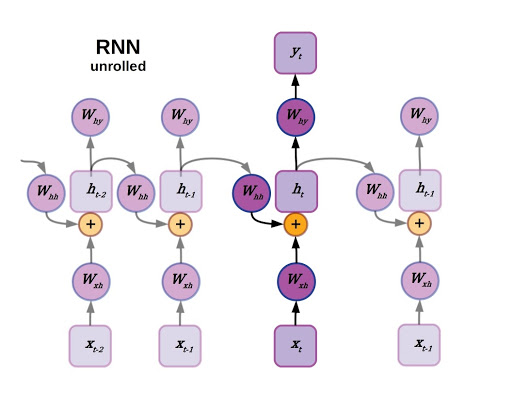
\includegraphics[width=0.7\textwidth]{RNN_Unrolled}
  \caption{An unrolled representation of a Recurrent Neural Network (RNN) showing how it processes input sequences by feeding the output of the previous time step as an additional input to the current time step. This allows the RNN to capture the temporal dependencies and learn patterns in sequential data.\cite{RNN:Unrolled}}
\end{figure}

One of the main limitations of traditional RNNs is the vanishing gradient problem, which occurs when the gradients of the parameters tend to decrease exponentially with the number of time steps.
This makes it difficult to train RNNs on long sequences.
To overcome this problem, variants of RNNs have been developed, such as Long Short-Term Memory (LSTM) and Gated Recurrent Unit (GRU).

LSTMs and GRUs are architectures that introduce gates that control the flow of information through the hidden state, allowing them to store information for longer periods of time. 

The main difference between LSTMs and GRUs is the number and complexity of the gates they use to control the flow of information.
LSTMs use three gates: an input gate, an output gate, and a forget gate.
The input gate controls the flow of new information into the cell, the output gate controls the flow of information out of the cell, and the forget gate controls the flow of information through the cell.

GRUs, on the other hand, use two gates: an update gate and a reset gate.
The update gate controls the flow of new information into the cell, and the reset gate controls the flow of information through the cell.
The update gate can be seen as a combination of the input gate and the forget gate in LSTM.

\begin{figure}[H]
  \centering
  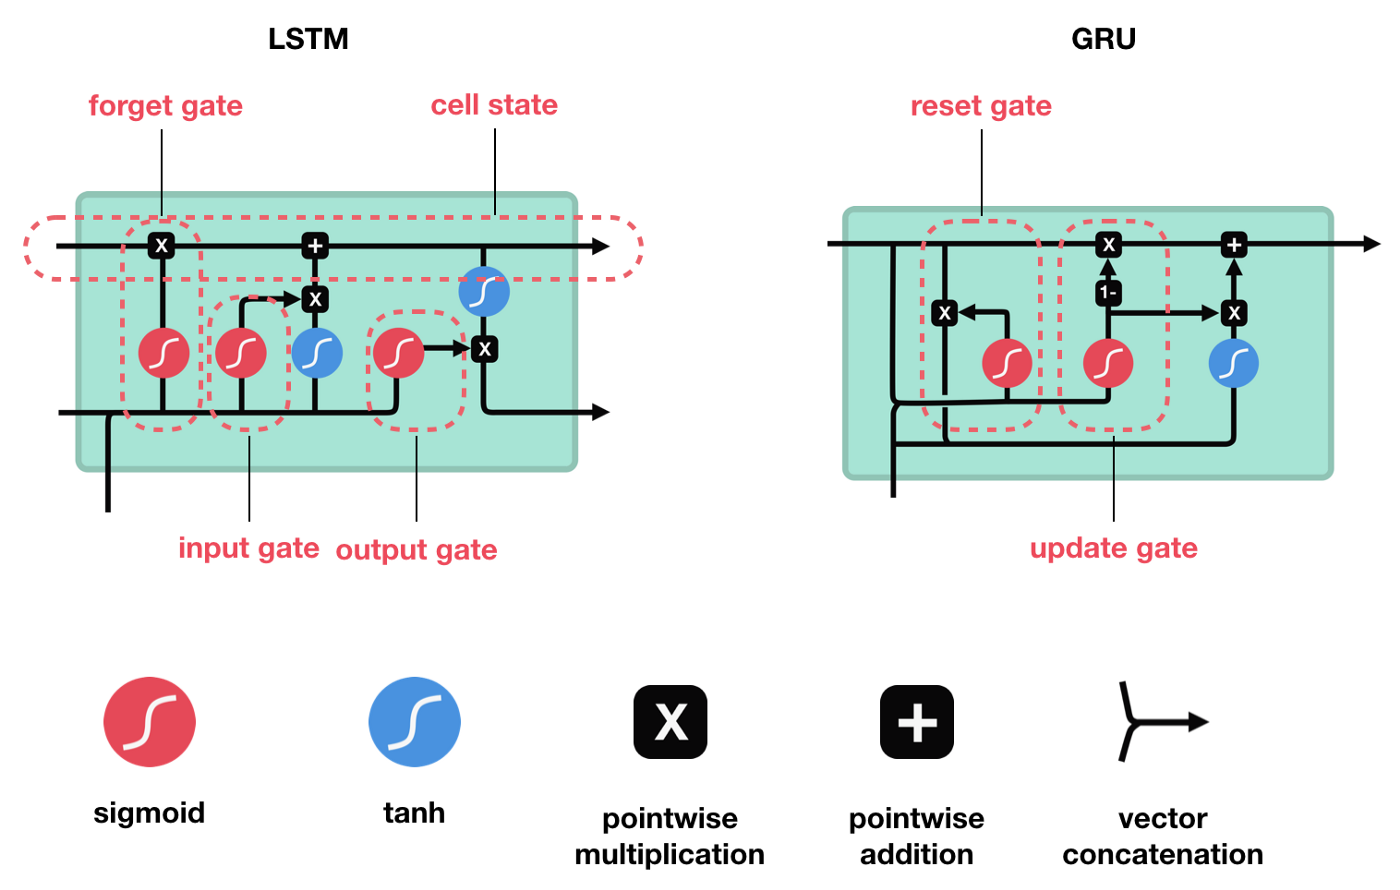
\includegraphics[width=0.6\textwidth]{lstm-gru}
  \caption{Visualization of LSTM and GRU cells \cite{phi}}
\end{figure}

In terms of performance, both LSTMs and GRUs have been shown to be effective at handling long-term dependencies in sequential data.
LSTMs have been used in a wide range of applications, such as language modeling, speech recognition, and machine translation, and have been shown to achieve state-of-the-art performance in many tasks.
GRUs, on the other hand, are more computationally efficient and have been used in applications such as natural language processing and speech recognition, and have been shown to achieve similar performance to LSTMs with fewer parameters.

In summary, Recurrent Neural Networks (RNNs) are a type of neural network designed to process sequential data.
They have a feedback loop that allows information to flow from one step of the sequence to the next, and a hidden state that contains information about past inputs.
However, traditional RNNs suffer from the vanishing gradient problem, which makes it difficult to train RNNs on long sequences.
To overcome this problem, variants of RNNs such as Long Short-Term Memory (LSTM) and Gated Recurrent Unit (GRU) have been developed. Both LSTMs and GRUs have been shown to be effective in solving a wide range of problems related to sequential data and have been applied to other areas as well.

\subsection{Generative adversarial networks}
Generative Adversarial Networks (GANs) \cite{goodfellow2014generative, mirza2014conditional} are a type of neural network architecture that is used for unsupervised learning.
They consist of two main components: a generator network and a discriminator network.
The generator network is trained to generate new data samples that are similar to a given training dataset, while the discriminator network is trained to distinguish between the generated samples and the real samples from the training dataset.

\begin{figure}[H]
  \centering
  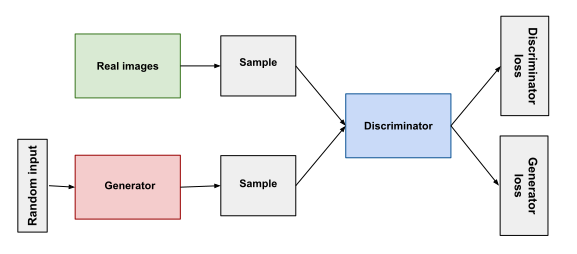
\includegraphics[width=0.8\textwidth]{gan}
  \caption{Overview of GAN structure \cite{googledevelopers}}
\end{figure}

The training process of GANs is based on a game-theoretic approach, where the generator and the discriminator compete against each other.
The generator tries to generate samples that are similar to the real samples, while the discriminator tries to correctly identify which samples are real and which are generated.
As training progresses, the generator gets better at generating realistic samples, while the discriminator gets better at identifying the generated samples.

One of the main advantages of GANs is that they can be used to generate high-quality images, videos, and other types of data.
They have been used in a wide range of applications, including image synthesis, image-to-image translation, style transfer, and video prediction. 
GANs have also been applied to other areas such as natural language processing, speech synthesis, and 3D object generation.

There are many variations of GANs, such as Wasserstein GANs \cite{arxiv.1701.07875}, which use the Wasserstein distance to measure the difference between the generated samples and the real samples, and Cycle GANs \cite{CycleGAN2017}, which are used for image-to-image translation.
There are also GANs that use different architectures, such as convolutional GANs and recurrent GANs.

Conditional GANs \cite{arxiv.1411.1784}, also known as cGANs, are a variant of GANs where both the generator and the discriminator are conditioned on some additional input, such as a class label or an image.
This allows the model to generate new samples that are conditioned on a specific class or attributes.
For example, it can generate images of a particular object or in a particular style.

In summary, Generative Adversarial Networks (GANs) are a type of neural network architecture used for unsupervised learning.
They consist of two main components: a generator network and a discriminator network.
The generator network is trained to generate new data samples that are similar to a given training data set, while the discriminator network is trained to distinguish between the generated samples and the real samples from the training data set.
GANs have many advantages, such as the ability to generate high-quality images, videos, and other types of data.
Conditional GANs are a variant of GANs where both the generator and the discriminator are conditioned on some additional input, such as a class label or an image, allowing the model to generate new samples conditioned on a specific class or attributes.
They have been used in a wide range of applications and have been applied to other areas such as natural language processing, speech synthesis, and 3D object generation.

\subsection{Attention is all you need}

The "Attention is All You Need" (AIAYN) \cite{vaswani} model, also known as the Transformer, is a neural network architecture introduced by Google researchers in 2017.
It is a type of encoder-decoder model that is primarily used for natural language processing tasks such as language translation, text summarization, and question answering.

The key innovation of Transformer is the use of self-attention mechanisms, which allow the model to focus on specific parts of the input while processing it.
Traditional encoder-decoder models use recurrent neural networks (RNNs) or convolutional neural networks (CNNs) to process the input sequentially, which can be slow and computationally expensive for long sequences.
In contrast, the Transformer uses self-attention mechanisms to process all parts of the input simultaneously, making it much faster and more efficient.

\begin{figure}[H]
  \centering
  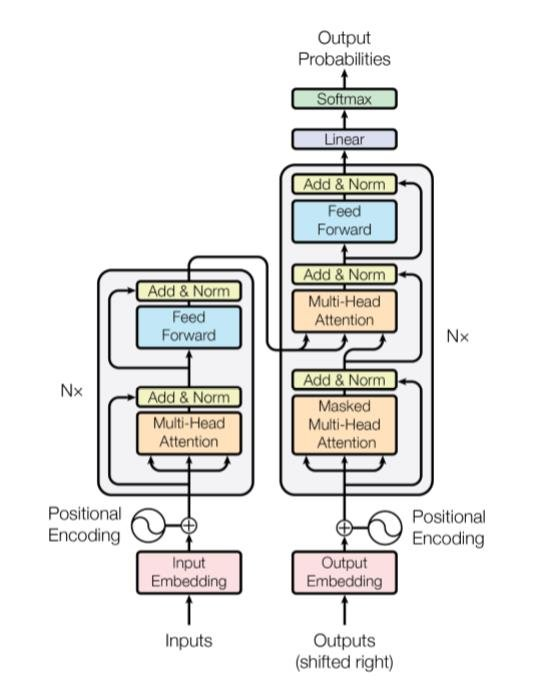
\includegraphics[width=0.7\textwidth]{transformer}
  \caption{The transformer model \cite{vaswani}}
\end{figure}

The Transformer architecture consists of an encoder and a decoder, which are both made up of multiple layers of self-attention and feed-forward neural networks.
The encoder takes in the input sequence and processes it using self-attention mechanisms, which allow the model to learn relationships between different parts of the input.
The decoder then takes the encoded representation and generates the output sequence.

The attention mechanism used in the Transformer is a type of dot-product attention, which calculates the similarity between different parts of the input.
The attention weights are then used to combine the different parts of the input to create a new representation.

One of the key advantages of the Transformer is its ability to handle input sequences of variable length, which is important for natural language processing tasks where the length of the input can vary widely.
In addition, the Transformer can be parallelized, allowing it to be trained and run on multiple GPUs or TPUs, resulting in faster training times.

In conclusion, the Attention is All You Need (AIAYN) model, also known as the Transformer, is a neural network architecture introduced in 2017.
The main innovation of the Transformer is the use of self-attention mechanisms, which allow the model to focus on certain parts of the input while processing it.
The Transformer architecture consists of an encoder and a decoder, both of which consist of multiple layers of self-attention and feed-forward neural networks.
The attention mechanism used in the Transformer is a type of point product attention that computes the similarity between different parts of the input.
One of the main advantages of the Transformer is its ability to handle variable-length input sequences, which is important for natural language processing tasks where the length of the input can vary greatly. 
In addition, the Transformer can be parallelized, allowing it to be trained and run on multiple GPUs or TPUs, resulting in faster training times.

